\documentclass{beamer}
\usetheme{metropolis}
\usepackage{graphicx}
\usepackage{amsmath}
\usepackage{tcolorbox}

\def\rcurs{{\mbox{$\resizebox{.16in}{.08in}{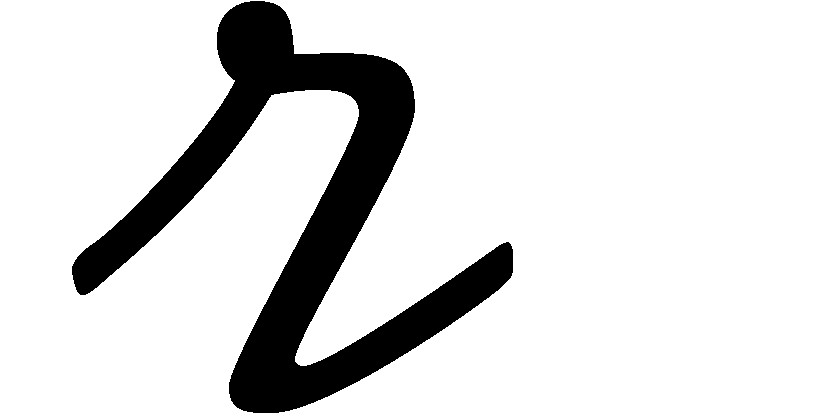
\includegraphics{ScriptR}}$}}}
\def\brcurs{{\mbox{$\resizebox{.16in}{.08in}{
\includegraphics{BoldR}}$}}}
\def\hrcurs{{\mbox{$\hat \brcurs$}}}

\title{Electromagnetc Theory: PHYS330}
\author{Jordan Hanson}
\institute{Whittier College Department of Physics and Astronomy}

\begin{document}
\maketitle

\section{Summary}

\begin{frame}{Week 2 Summary}
\begin{enumerate}
\item Homework discussions
\begin{itemize}
\item Proofs!  Glorious proofs.
\item Exercises with \textit{checking} fundamental theorems
\end{itemize}
\item Electrostatics and Coulomb forces
\begin{itemize}
\item Charge distributions, superposition, and the Coulomb force
\item A note about the \textit{far-field}
\item Setting up integrals, taking limits, checking units
\item The divergence of electric fields
\item The curl of electric fields
\end{itemize}
\item Electric Potential
\begin{itemize}
\item Definitions, fundamental theorem for gradients
\item Reference points
\item Laplace equation ...
\end{itemize}
\item Work, energy, and conductors
\end{enumerate}
\end{frame}

\section{Homework}

\begin{frame}{Homework, Week 2}
Unlike last week, these exercises come from \textit{within} the chapter.  Ideally, you should look at all of the problems within the chapter as you study.
\begin{itemize}
\item Exercise 2.5
\item Exercise 2.6
\item Exercise 2.9
\item Exercise 2.12
\item Exercsie 2.16
\item Exercise 2.18
\item Exercise 2.25
\item Exercise 2.29
\end{itemize}
\end{frame}

\section{Charge distributions, Superposition, and the Coulomb Force}

\begin{frame}{Charge distributions, Superposition, and the Coulomb Force}
\begin{figure}
\centering
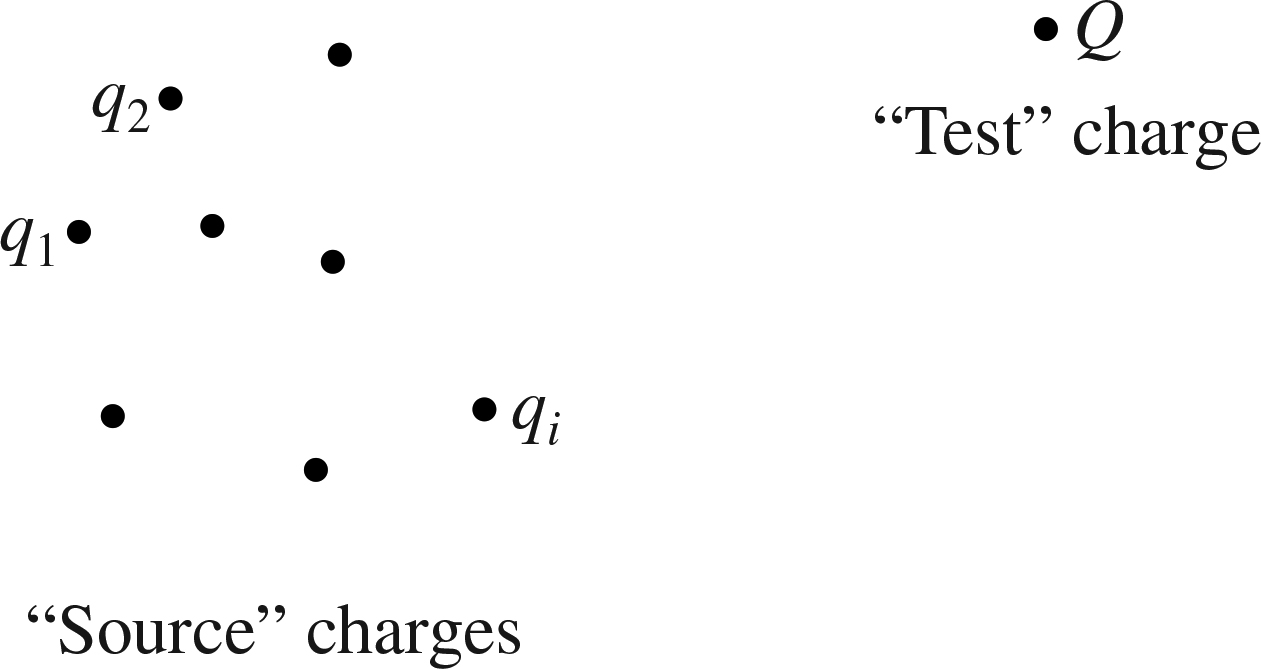
\includegraphics[width=5cm]{figures/2_1.jpg}
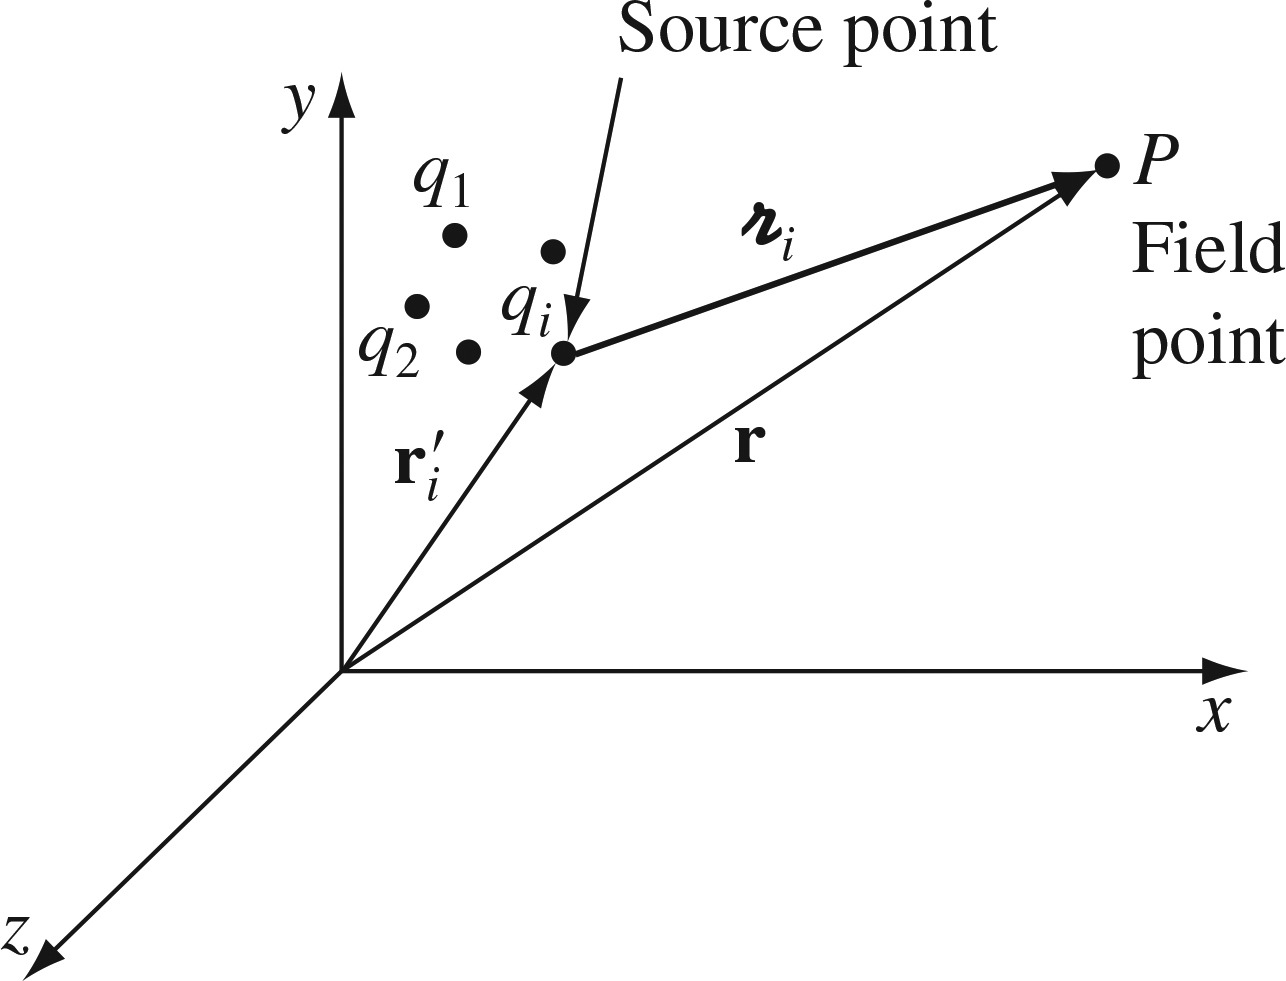
\includegraphics[width=5cm]{figures/2_3.jpg}
\caption{\label{fig:2_1} The basic problem of electrostatics. Note the definition of the separation vector, and the vectors to the field point and to all the source charges.}
\end{figure}
\end{frame}

\begin{frame}{Charge distributions, Superposition, and the Coulomb Force}
\begin{figure}
\centering
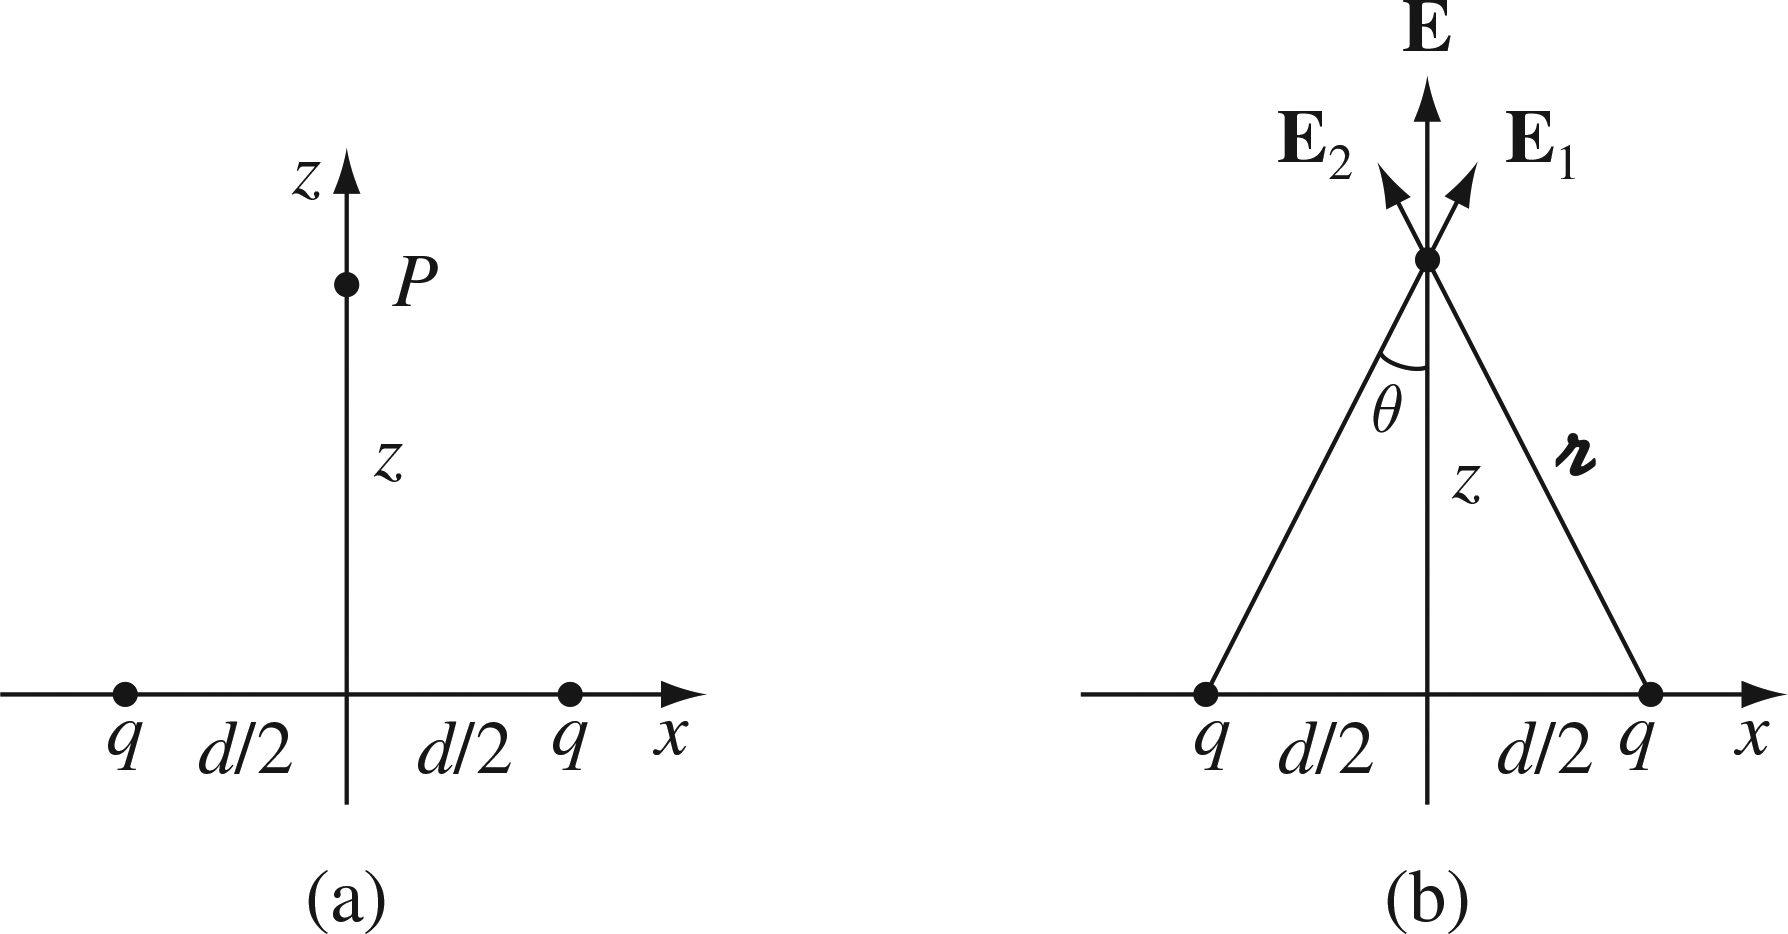
\includegraphics[width=10cm]{figures/2_4.jpg}
\caption{\label{fig:2_4} Begin with a dipole, and then a \textit{physical} dipole.}
\end{figure}
\end{frame}

\begin{frame}{Charge distributions, Superposition, and the Coulomb Force}
\begin{figure}
\centering
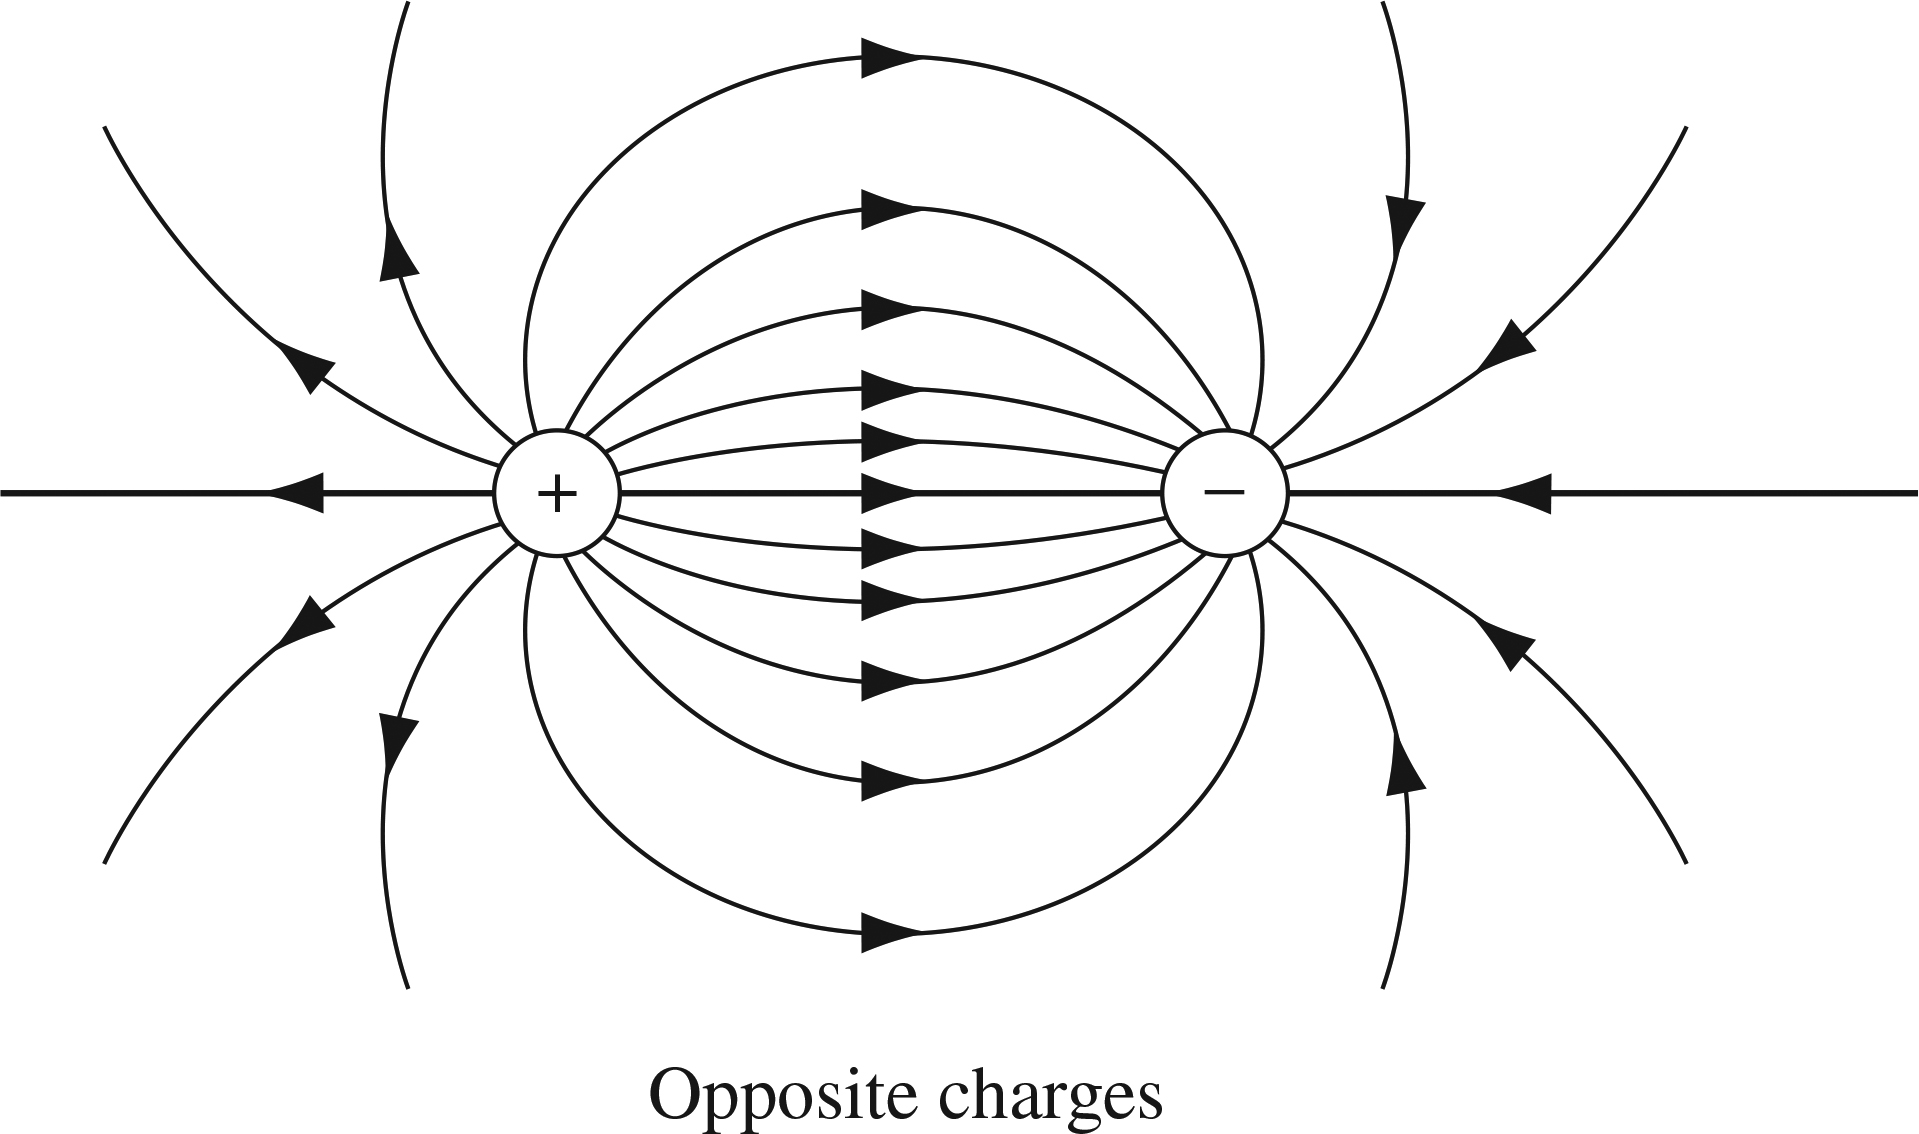
\includegraphics[width=10cm]{figures/2_13.jpg}
\caption{\label{fig:2_13} Field of a \textit{physical} dipole.}
\end{figure}
\end{frame}

\begin{frame}{Charge distributions, Superposition, and the Coulomb Force}
\begin{figure}
\centering
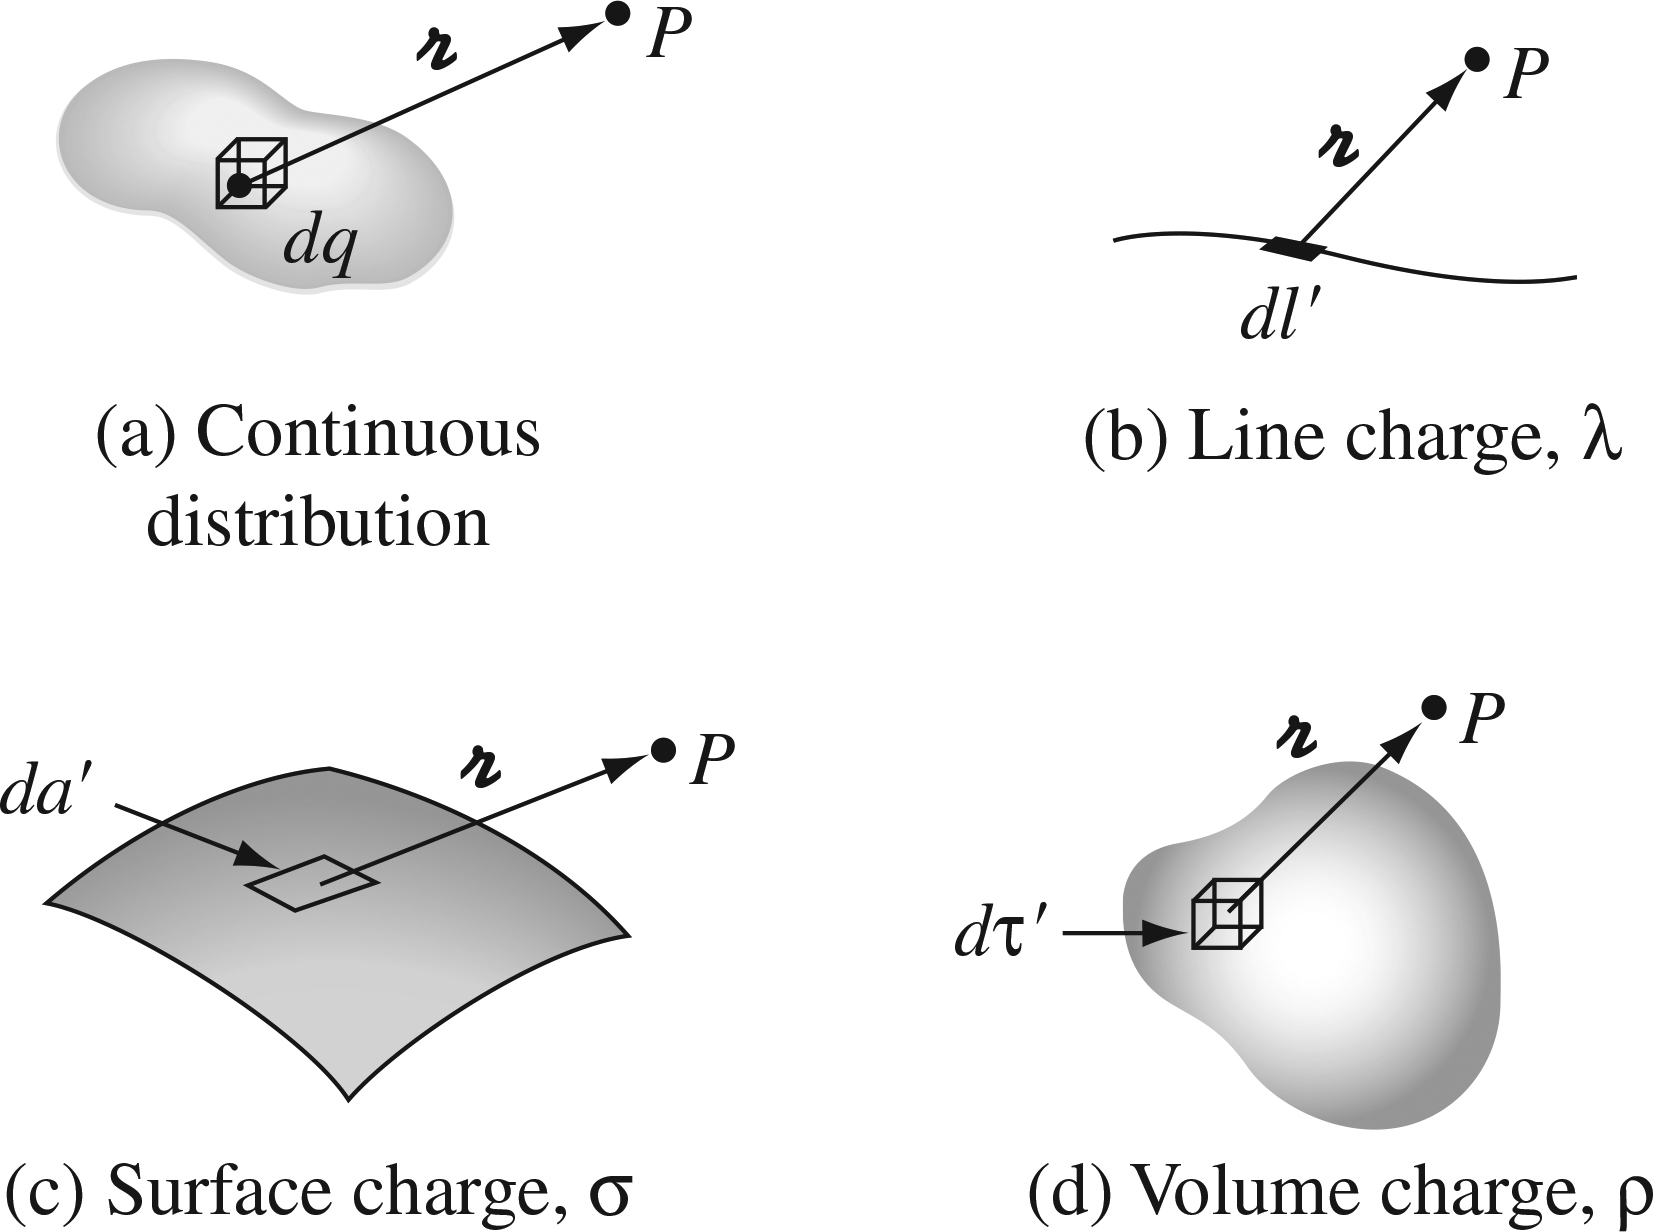
\includegraphics[width=8cm]{figures/2_5.jpg}
\caption{\label{fig:2_5} The continuous limit implies a variety of symmetries and geometries over which we integrate, rather than sum.}
\end{figure}
\end{frame}

\begin{frame}{Charge distributions, Superposition, and the Coulomb Force}
\begin{figure}
\centering
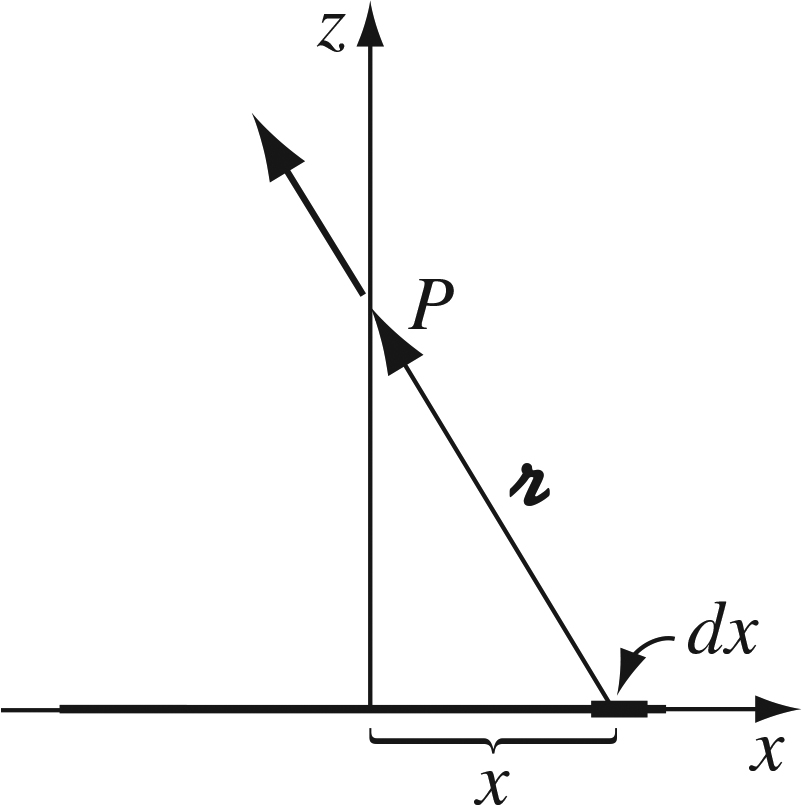
\includegraphics[width=6cm]{figures/2_6.jpg}
\caption{\label{fig:2_6} A coninuous line density of charge.  Integration yields the electric field.}
\end{figure}
\end{frame}

\begin{frame}{Charge distributions, Superposition, and the Coulomb Force}
\alert{Useful calculations:}
\begin{enumerate}
\item Continuous line charge, length $L$.
\item Continuous plane of charge, radius $R$.
\item Loop of charge, radius $R$, a distance $z$ above the center.
\end{enumerate}
Why are these interesting?  One example is that these shapes are used as \textit{antennas}.  Give some alternating current at the right voltage and impedance to a shape of metal, then you've got your antenna that radiates a certain way. \\ \vspace{1cm}
\textbf{Professor do these examples.}\footnote{Remember from PHYS180? Remember? Yeah...good times.}
\end{frame}

\section{A Note about the Far-Field}

\begin{frame}{The Far-Field}
\small
One way to express the \textbf{\alert{far-field}} approximation (compare to Fraunhofer and Fresnel limits in diffraction):
\begin{align}
\vec{r} &= \vec{r'} + \vec{\rcurs} \\
\vec{\rcurs} &= \vec{r} - \vec{r'} \\
\rcurs &= \sqrt{r^2 - 2 \vec{r} \cdot \vec{r'} + r'^2} \\
\rcurs &= r\sqrt{1 - 2 \vec{r} \cdot \vec{r'} r^{-2} + r'^2 r^{-2}} \\
\rcurs &\approx r\sqrt{1 - 2 \vec{r} \cdot \vec{r'} r^{-2}} \\
\rcurs &\approx r\left(1 - \vec{r} \cdot \vec{r'} r^{-2}\right) \\
\rcurs &\approx r\left(1 - \hat{r} \cdot \vec{r'} r^{-1}\right) \\
\rcurs &\approx r - \hat{r} \cdot \vec{r'}
\end{align}
\end{frame}

\section{The Divergence of $\vec{E}$-fields}

\begin{frame}{The Divergence of $\vec{E}$-fields}
\begin{figure}
\centering
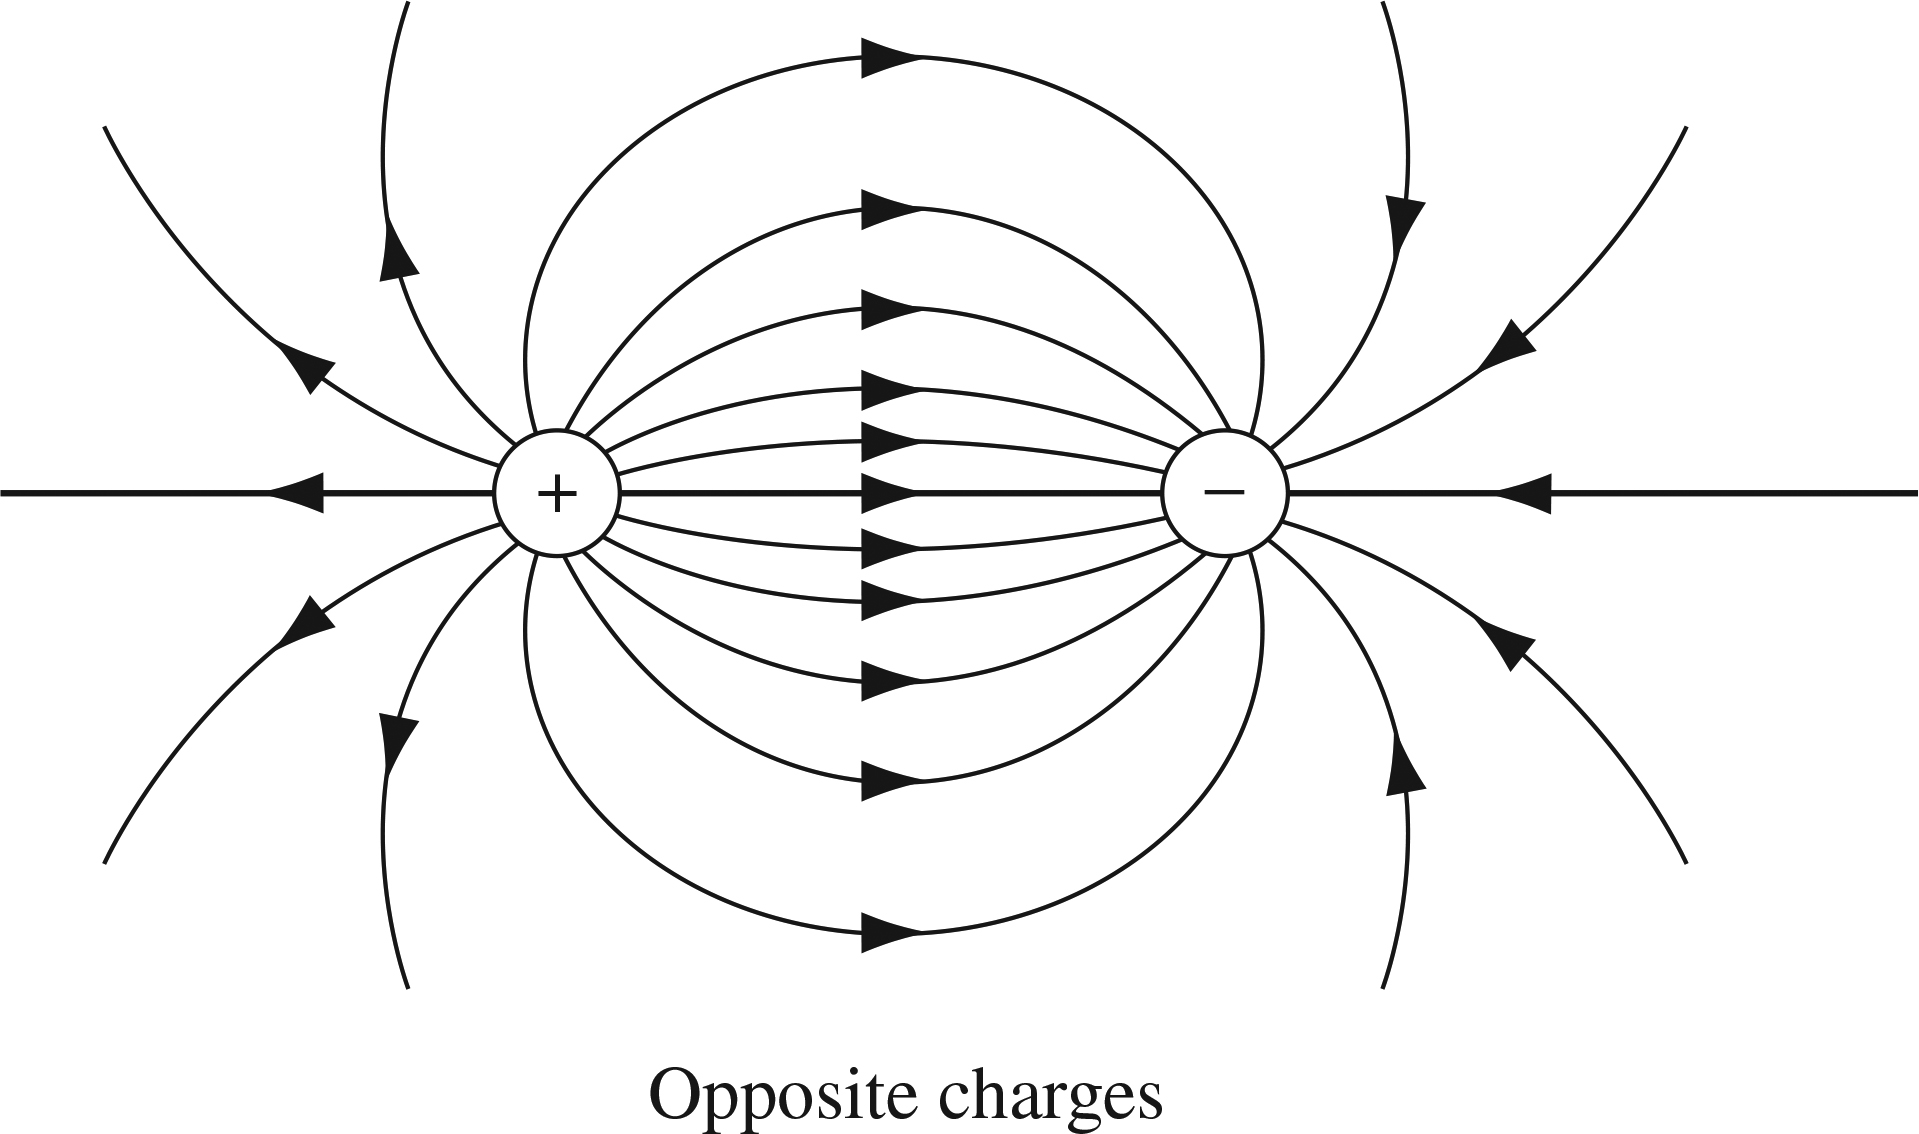
\includegraphics[width=5cm]{figures/2_13.jpg}
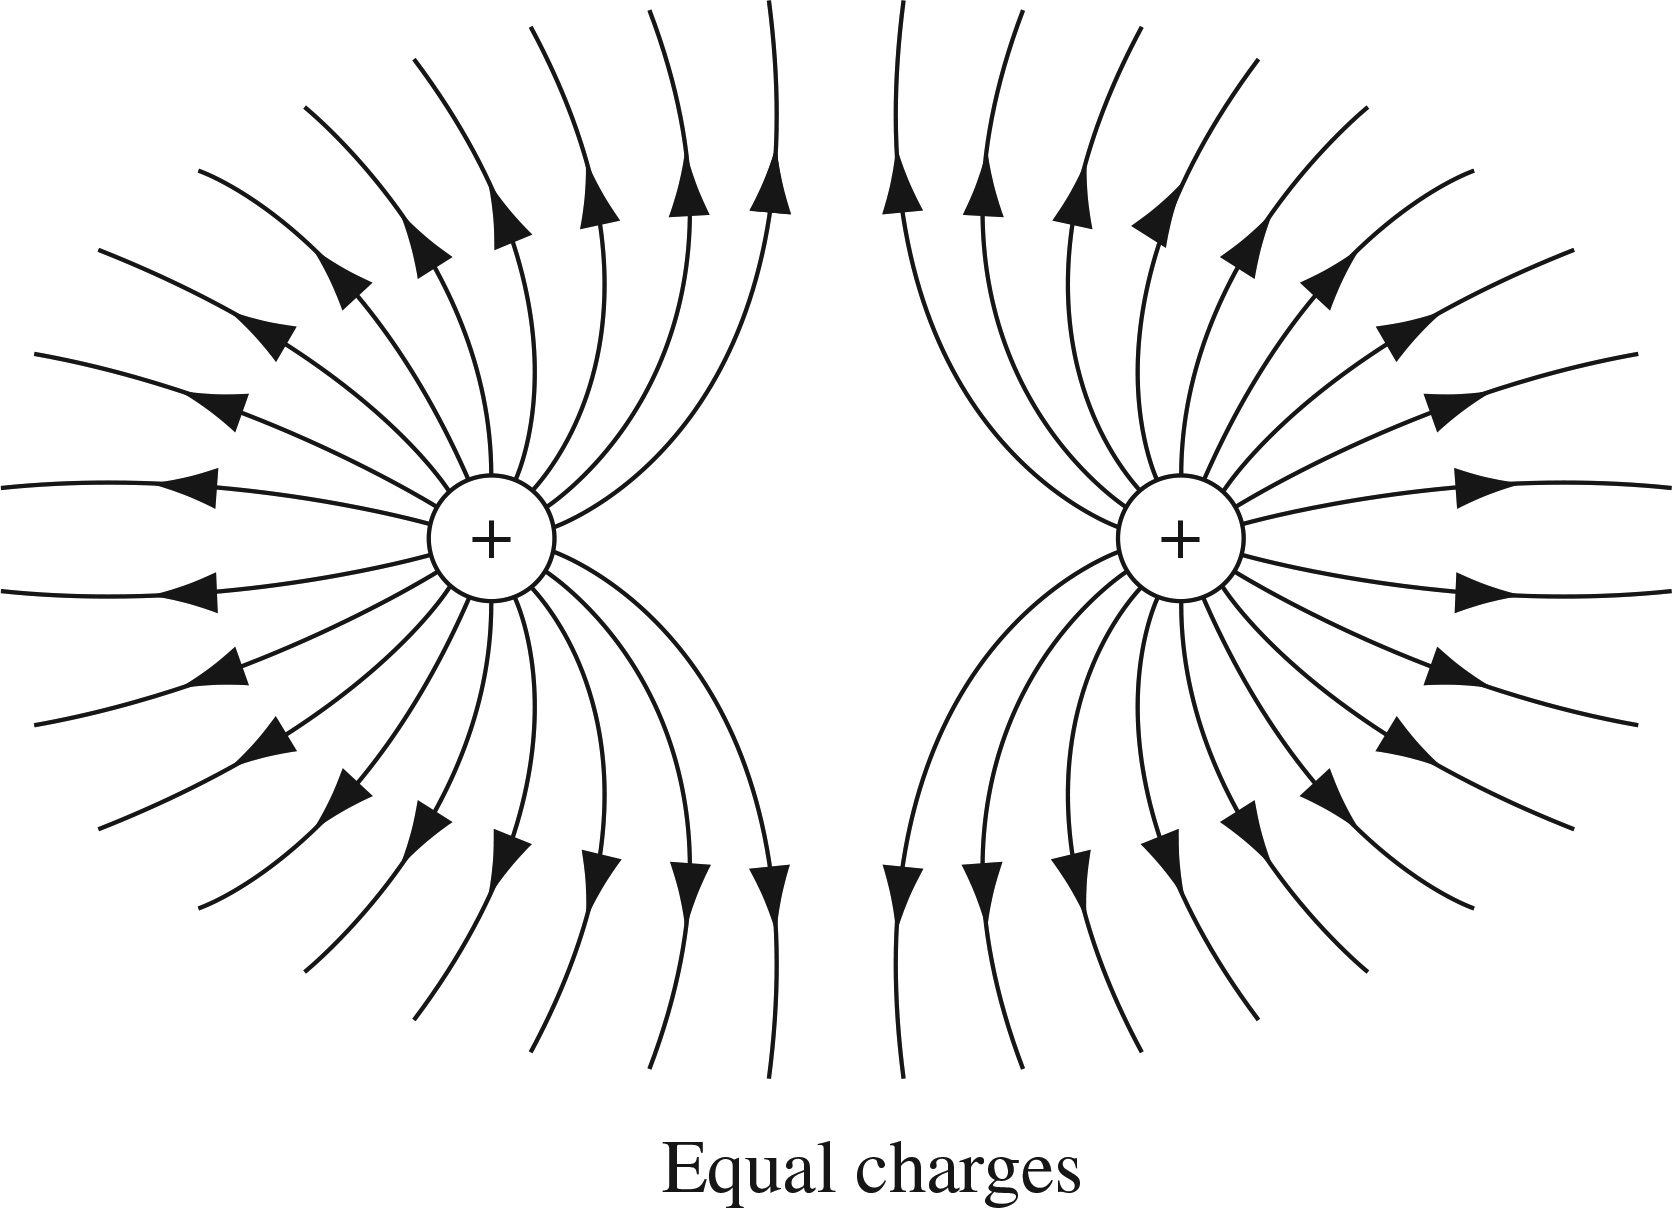
\includegraphics[width=4cm]{figures/2_14.jpg}
\caption{\label{fig:fieldLines} Field lines are an important theoretical concept.}
\end{figure}
\end{frame}

\begin{frame}{The Divergence of $\vec{E}$-fields}
\begin{figure}
\centering
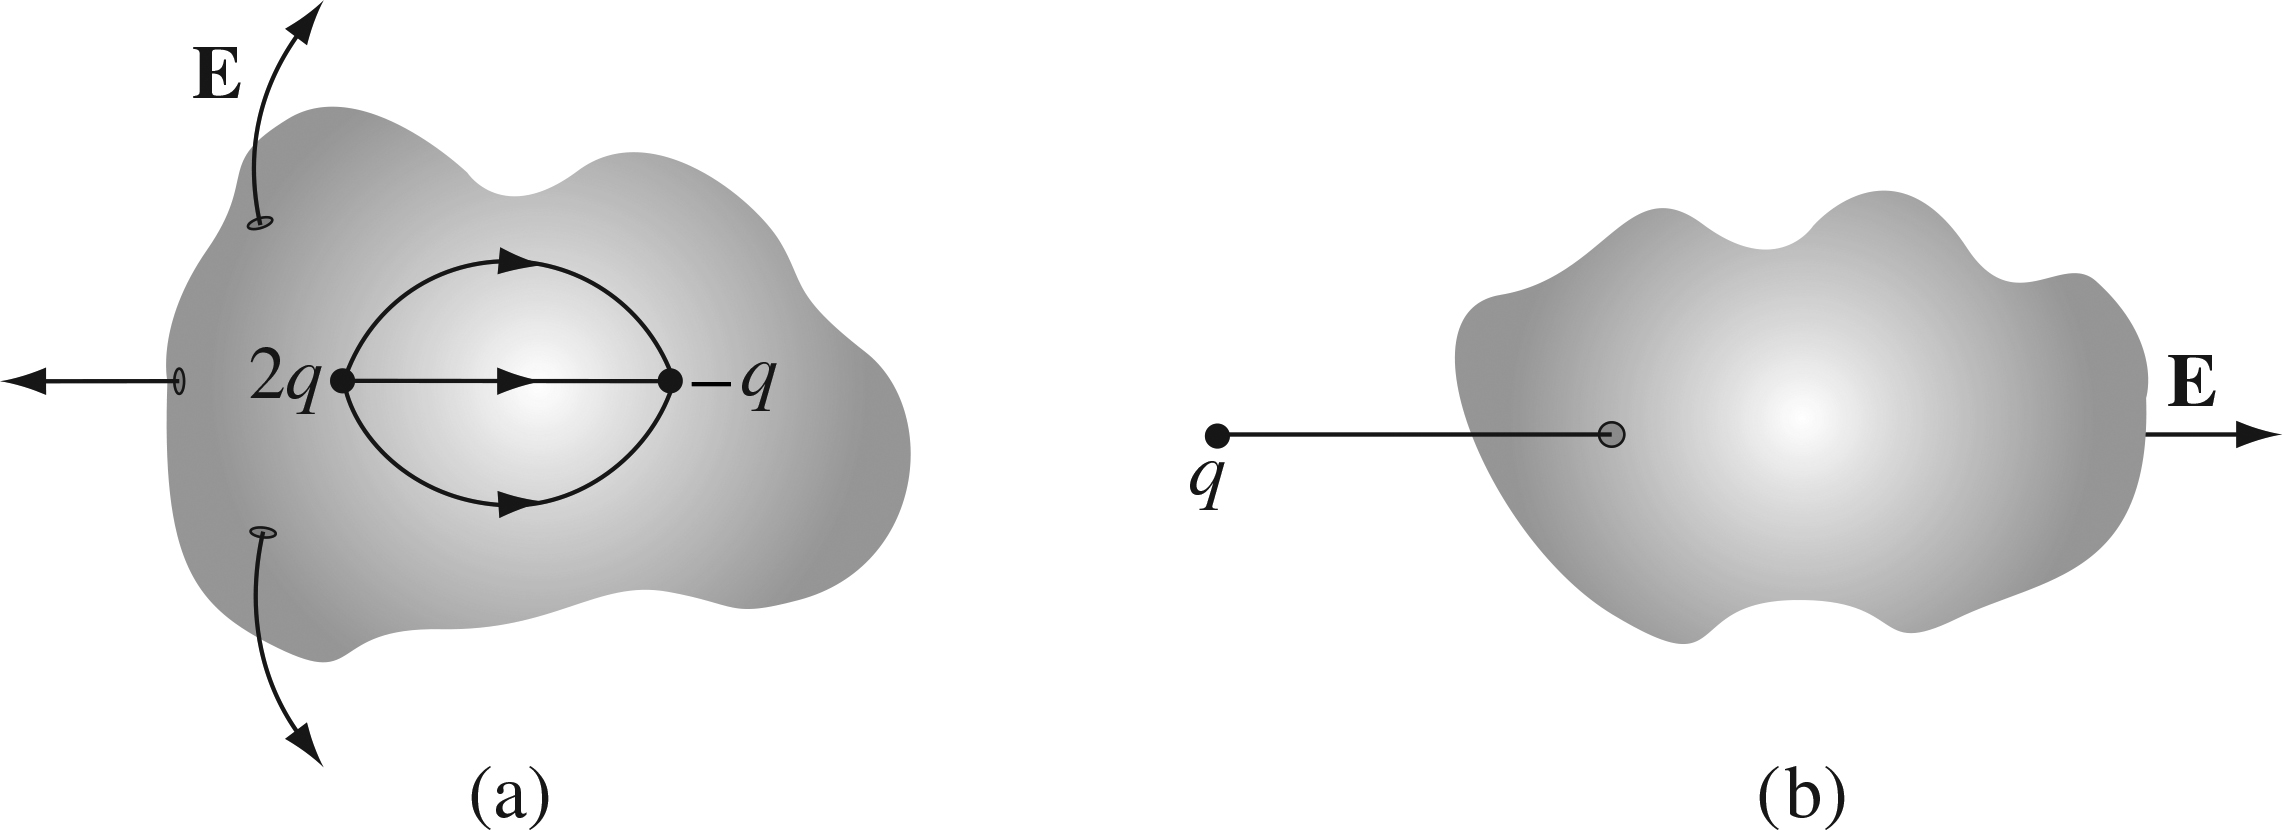
\includegraphics[width=10cm]{figures/2_16.jpg}
\caption{\label{fig:fieldLines2} The concept of a closed Gaussian surface.}
\end{figure}
\end{frame}

\begin{frame}{The Divergence of $\vec{E}$-fields}
\begin{equation}
\boxed{
\oint \vec{E_i} \cdot d\vec{a} = \frac{1}{4\pi \epsilon_0} \int_0^{\pi} \int_0^{2\pi} \frac{q_i\hat{r}}{r^2} \cdot r^2 \sin\theta d\theta d\phi \hat{r} = \frac{q_i}{\epsilon_0}
}
\end{equation}
\begin{align}
\vec{E} =& \sum_{i=1}^n \vec{E}_i \\
\oint \vec{E} \cdot d\vec{a} =& \sum_{i=1}^n \left(\oint \vec{E}_i \cdot d\vec{a}\right) \\
\oint \vec{E} \cdot d\vec{a} =& \sum_{i=1}^n \left( \frac{q_i}{\epsilon_0} \right) \\
\oint \vec{E} \cdot d\vec{a} =& \frac{Q_{tot}}{\epsilon_0}
\end{align}
\alert{Gauss' Law: the total flux is proportional to the contained charge.}
\end{frame}

\begin{frame}{The Divergence of $\vec{E}$-fields}
The divergence theorem:
\begin{equation}
\oint_{\mathcal{S}} \vec{E} \cdot d\vec{a} = \int_{\mathcal{V}} (\nabla \cdot \vec{E}) d\tau
\end{equation}
Remark that the total charge is the integral over the 3D charge density:
\begin{equation}
\frac{Q_{tot}}{\epsilon_0} = \frac{1}{\epsilon_0}\int_{\mathcal{V}} \rho d\tau
\end{equation}
This implies
\begin{equation}
\oint_{\mathcal{S}} \vec{E} \cdot d\vec{a} = \int_{\mathcal{V}} (\nabla \cdot \vec{E}) d\tau = \frac{1}{\epsilon_0}\int_{\mathcal{V}} \rho d\tau
\end{equation}
Looking at the last two expressions:
\begin{equation}
\boxed{
\nabla \cdot \vec{E} = \frac{\rho}{\epsilon_0}
}
\end{equation}
\end{frame}

\begin{frame}{The Divergence of $\vec{E}$-fields}
\textit{Differential form} of Gauss' Law:
\begin{equation}
\boxed{
\nabla \cdot \vec{E} = \frac{\rho}{\epsilon_0}
}
\end{equation}
Consider a different argument:
\begin{align}
\vec{E} =& \frac{1}{4\pi\epsilon_0} \int \frac{\hat{\hrcurs}}{\rcurs^2} \rho(\vec{r}') d\tau' \label{eq:E} \\
\nabla \cdot \vec{E} =& \frac{1}{4\pi\epsilon_0} \int \nabla \cdot \left(\frac{\hat{\hrcurs}}{\rcurs^2} \right)\rho(\vec{r}') d\tau' \\
\nabla \cdot \vec{E} =& \frac{1}{4\pi\epsilon_0} \int 4\pi \delta^3(\brcurs)\rho(\vec{r}') d\tau' \\
\nabla \cdot \vec{E} =& \frac{4\pi}{4\pi\epsilon_0} \int \delta^3(\vec{r} - \vec{r}')\rho(\vec{r}') d\tau' \\
\nabla \cdot \vec{E} =& \rho(\vec{r})/\epsilon_0
\end{align}
\end{frame}

\begin{frame}{The Divergence of $\vec{E}$-fields}
\small
(Refresh with delta-functions): Use this charge distribution and Eq. \ref{eq:E} to find the $\vec{E}$-field.
\begin{equation}
\rho(\vec{r}') = q \delta^3(\vec{r}' - x\hat{x}) - q \delta^3(\vec{r}' + x\hat{x})
\end{equation} 
\vspace{7cm}

\end{frame}

\end{document}
